
%% bare_conf.tex
%% V1.3
%% 2007/01/11
%% by Michael Shell
%% See:
%% http://www.michaelshell.org/
%% for current contact information.
%%
%% This is a skeleton file demonstrating the use of IEEEtran.cls
%% (requires IEEEtran.cls version 1.7 or later) with an IEEE conference paper.
%%
%% Support sites:
%% http://www.michaelshell.org/tex/ieeetran/
%% http://www.ctan.org/tex-archive/macros/latex/contrib/IEEEtran/
%% and
%% http://www.ieee.org/

%%*************************************************************************
%% Legal Notice:
%% This code is offered as-is without any warranty either expressed or
%% implied; without even the implied warranty of MERCHANTABILITY or
%% FITNESS FOR A PARTICULAR PURPOSE! 
%% User assumes all risk.
%% In no event shall IEEE or any contributor to this code be liable for
%% any damages or losses, including, but not limited to, incidental,
%% consequential, or any other damages, resulting from the use or misuse
%% of any information contained here.
%%
%% All comments are the opinions of their respective authors and are not
%% necessarily endorsed by the IEEE.
%%
%% This work is distributed under the LaTeX Project Public License (LPPL)
%% ( http://www.latex-project.org/ ) version 1.3, and may be freely used,
%% distributed and modified. A copy of the LPPL, version 1.3, is included
%% in the base LaTeX documentation of all distributions of LaTeX released
%% 2003/12/01 or later.
%% Retain all contribution notices and credits.
%% ** Modified files should be clearly indicated as such, including  **
%% ** renaming them and changing author support contact information. **
%%
%% File list of work: IEEEtran.cls, IEEEtran_HOWTO.pdf, bare_adv.tex,
%%                    bare_conf.tex, bare_jrnl.tex, bare_jrnl_compsoc.tex
%%*************************************************************************

% *** Authors should verify (and, if needed, correct) their LaTeX system  ***
% *** with the testflow diagnostic prior to trusting their LaTeX platform ***
% *** with production work. IEEE's font choices can trigger bugs that do  ***
% *** not appear when using other class files.                            ***
% The testflow support page is at:
% http://www.michaelshell.org/tex/testflow/



% Note that the a4paper option is mainly intended so that authors in
% countries using A4 can easily print to A4 and see how their papers will
% look in print - the typesetting of the document will not typically be
% affected with changes in paper size (but the bottom and side margins will).
% Use the testflow package mentioned above to verify correct handling of
% both paper sizes by the user's LaTeX system.
%
% Also note that the "draftcls" or "draftclsnofoot", not "draft", option
% should be used if it is desired that the figures are to be displayed in
% draft mode.
%
\documentclass[conference]{IEEEtran}
\usepackage{blindtext, graphicx}
\usepackage{hyperref}
\usepackage{caption}
\usepackage{amsmath}
\usepackage{csquotes}
\usepackage[nocaptions]{vntex}
\usepackage{url}
\usepackage[table,xcdraw]{xcolor}
\newcommand\abs[1]{\left|#1\right|}
% Add the compsoc option for Computer Society conferences.
%
% If IEEEtran.cls has not been installed into the LaTeX system files,
% manually specify the path to it like:
% \documentclass[conference]{../sty/IEEEtran}





% Some very useful LaTeX packages include:
% (uncomment the ones you want to load)


% *** MISC UTILITY PACKAGES ***
%
%\usepackage{ifpdf}
% Heiko Oberdiek's ifpdf.sty is very useful if you need conditional
% compilation based on whether the output is pdf or dvi.
% usage:
% \ifpdf
%   % pdf code
% \else
%   % dvi code
% \fi
% The latest version of ifpdf.sty can be obtained from:
% http://www.ctan.org/tex-archive/macros/latex/contrib/oberdiek/
% Also, note that IEEEtran.cls V1.7 and later provides a builtin
% \ifCLASSINFOpdf conditional that works the same way.
% When switching from latex to pdflatex and vice-versa, the compiler may
% have to be run twice to clear warning/error messages.






% *** CITATION PACKAGES ***
%
%\usepackage{cite}
% cite.sty was written by Donald Arseneau
% V1.6 and later of IEEEtran pre-defines the format of the cite.sty package
% \cite{} output to follow that of IEEE. Loading the cite package will
% result in citation numbers being automatically sorted and properly
% "compressed/ranged". e.g., [1], [9], [2], [7], [5], [6] without using
% cite.sty will become [1], [2], [5]--[7], [9] using cite.sty. cite.sty's
% \cite will automatically add leading space, if needed. Use cite.sty's
% noadjust option (cite.sty V3.8 and later) if you want to turn this off.
% cite.sty is already installed on most LaTeX systems. Be sure and use
% version 4.0 (2003-05-27) and later if using hyperref.sty. cite.sty does
% not currently provide for hyperlinked citations.
% The latest version can be obtained at:
% http://www.ctan.org/tex-archive/macros/latex/contrib/cite/
% The documentation is contained in the cite.sty file itself.






% *** GRAPHICS RELATED PACKAGES ***
%
\ifCLASSINFOpdf
  % \usepackage[pdftex]{graphicx}
  % declare the path(s) where your graphic files are
  % \graphicspath{{../pdf/}{../jpeg/}}
  % and their extensions so you won't have to specify these with
  % every instance of \includegraphics
  % \DeclareGraphicsExtensions{.pdf,.jpeg,.png}
\else
  % or other class option (dvipsone, dvipdf, if not using dvips). graphicx
  % will default to the driver specified in the system graphics.cfg if no
  % driver is specified.
  % \usepackage[dvips]{graphicx}
  % declare the path(s) where your graphic files are
  % \graphicspath{{../eps/}}
  % and their extensions so you won't have to specify these with
  % every instance of \includegraphics
  % \DeclareGraphicsExtensions{.eps}
\fi
% graphicx was written by David Carlisle and Sebastian Rahtz. It is
% required if you want graphics, photos, etc. graphicx.sty is already
% installed on most LaTeX systems. The latest version and documentation can
% be obtained at: 
% http://www.ctan.org/tex-archive/macros/latex/required/graphics/
% Another good source of documentation is "Using Imported Graphics in
% LaTeX2e" by Keith Reckdahl which can be found as epslatex.ps or
% epslatex.pdf at: http://www.ctan.org/tex-archive/info/
%
% latex, and pdflatex in dvi mode, support graphics in encapsulated
% postscript (.eps) format. pdflatex in pdf mode supports graphics
% in .pdf, .jpeg, .png and .mps (metapost) formats. Users should ensure
% that all non-photo figures use a vector format (.eps, .pdf, .mps) and
% not a bitmapped formats (.jpeg, .png). IEEE frowns on bitmapped formats
% which can result in "jaggedy"/blurry rendering of lines and letters as
% well as large increases in file sizes.
%
% You can find documentation about the pdfTeX application at:
% http://www.tug.org/applications/pdftex





% *** MATH PACKAGES ***
%
%\usepackage[cmex10]{amsmath}
% A popular package from the American Mathematical Society that provides
% many useful and powerful commands for dealing with mathematics. If using
% it, be sure to load this package with the cmex10 option to ensure that
% only type 1 fonts will utilized at all point sizes. Without this option,
% it is possible that some math symbols, particularly those within
% footnotes, will be rendered in bitmap form which will result in a
% document that can not be IEEE Xplore compliant!
%
% Also, note that the amsmath package sets \interdisplaylinepenalty to 10000
% thus preventing page breaks from occurring within multiline equations. Use:
%\interdisplaylinepenalty=2500
% after loading amsmath to restore such page breaks as IEEEtran.cls normally
% does. amsmath.sty is already installed on most LaTeX systems. The latest
% version and documentation can be obtained at:
% http://www.ctan.org/tex-archive/macros/latex/required/amslatex/math/





% *** SPECIALIZED LIST PACKAGES ***
%
%\usepackage{algorithmic}
% algorithmic.sty was written by Peter Williams and Rogerio Brito.
% This package provides an algorithmic environment fo describing algorithms.
% You can use the algorithmic environment in-text or within a figure
% environment to provide for a floating algorithm. Do NOT use the algorithm
% floating environment provided by algorithm.sty (by the same authors) or
% algorithm2e.sty (by Christophe Fiorio) as IEEE does not use dedicated
% algorithm float types and packages that provide these will not provide
% correct IEEE style captions. The latest version and documentation of
% algorithmic.sty can be obtained at:
% http://www.ctan.org/tex-archive/macros/latex/contrib/algorithms/
% There is also a support site at:
% http://algorithms.berlios.de/index.html
% Also of interest may be the (relatively newer and more customizable)
% algorithmicx.sty package by Szasz Janos:
% http://www.ctan.org/tex-archive/macros/latex/contrib/algorithmicx/




% *** ALIGNMENT PACKAGES ***
%
%\usepackage{array}
% Frank Mittelbach's and David Carlisle's array.sty patches and improves
% the standard LaTeX2e array and tabular environments to provide better
% appearance and additional user controls. As the default LaTeX2e table
% generation code is lacking to the point of almost being broken with
% respect to the quality of the end results, all users are strongly
% advised to use an enhanced (at the very least that provided by array.sty)
% set of table tools. array.sty is already installed on most systems. The
% latest version and documentation can be obtained at:
% http://www.ctan.org/tex-archive/macros/latex/required/tools/


%\usepackage{mdwmath}
%\usepackage{mdwtab}
% Also highly recommended is Mark Wooding's extremely powerful MDW tools,
% especially mdwmath.sty and mdwtab.sty which are used to format equations
% and tables, respectively. The MDWtools set is already installed on most
% LaTeX systems. The lastest version and documentation is available at:
% http://www.ctan.org/tex-archive/macros/latex/contrib/mdwtools/


% IEEEtran contains the IEEEeqnarray family of commands that can be used to
% generate multiline equations as well as matrices, tables, etc., of high
% quality.


%\usepackage{eqparbox}
% Also of notable interest is Scott Pakin's eqparbox package for creating
% (automatically sized) equal width boxes - aka "natural width parboxes".
% Available at:
% http://www.ctan.org/tex-archive/macros/latex/contrib/eqparbox/





% *** SUBFIGURE PACKAGES ***
%\usepackage[tight,footnotesize]{subfigure}
% subfigure.sty was written by Steven Douglas Cochran. This package makes it
% easy to put subfigures in your figures. e.g., "Figure 1a and 1b". For IEEE
% work, it is a good idea to load it with the tight package option to reduce
% the amount of white space around the subfigures. subfigure.sty is already
% installed on most LaTeX systems. The latest version and documentation can
% be obtained at:
% http://www.ctan.org/tex-archive/obsolete/macros/latex/contrib/subfigure/
% subfigure.sty has been superceeded by subfig.sty.



%\usepackage[caption=false]{caption}
%\usepackage[font=footnotesize]{subfig}
% subfig.sty, also written by Steven Douglas Cochran, is the modern
% replacement for subfigure.sty. However, subfig.sty requires and
% automatically loads Axel Sommerfeldt's caption.sty which will override
% IEEEtran.cls handling of captions and this will result in nonIEEE style
% figure/table captions. To prevent this problem, be sure and preload
% caption.sty with its "caption=false" package option. This is will preserve
% IEEEtran.cls handing of captions. Version 1.3 (2005/06/28) and later 
% (recommended due to many improvements over 1.2) of subfig.sty supports
% the caption=false option directly:
%\usepackage[caption=false,font=footnotesize]{subfig}
%
% The latest version and documentation can be obtained at:
% http://www.ctan.org/tex-archive/macros/latex/contrib/subfig/
% The latest version and documentation of caption.sty can be obtained at:
% http://www.ctan.org/tex-archive/macros/latex/contrib/caption/




% *** FLOAT PACKAGES ***
%
%\usepackage{fixltx2e}
% fixltx2e, the successor to the earlier fix2col.sty, was written by
% Frank Mittelbach and David Carlisle. This package corrects a few problems
% in the LaTeX2e kernel, the most notable of which is that in current
% LaTeX2e releases, the ordering of single and double column floats is not
% guaranteed to be preserved. Thus, an unpatched LaTeX2e can allow a
% single column figure to be placed prior to an earlier double column
% figure. The latest version and documentation can be found at:
% http://www.ctan.org/tex-archive/macros/latex/base/



%\usepackage{stfloats}
% stfloats.sty was written by Sigitas Tolusis. This package gives LaTeX2e
% the ability to do double column floats at the bottom of the page as well
% as the top. (e.g., "\begin{figure*}[!b]" is not normally possible in
% LaTeX2e). It also provides a command:
%\fnbelowfloat
% to enable the placement of footnotes below bottom floats (the standard
% LaTeX2e kernel puts them above bottom floats). This is an invasive package
% which rewrites many portions of the LaTeX2e float routines. It may not work
% with other packages that modify the LaTeX2e float routines. The latest
% version and documentation can be obtained at:
% http://www.ctan.org/tex-archive/macros/latex/contrib/sttools/
% Documentation is contained in the stfloats.sty comments as well as in the
% presfull.pdf file. Do not use the stfloats baselinefloat ability as IEEE
% does not allow \baselineskip to stretch. Authors submitting work to the
% IEEE should note that IEEE rarely uses double column equations and
% that authors should try to avoid such use. Do not be tempted to use the
% cuted.sty or midfloat.sty packages (also by Sigitas Tolusis) as IEEE does
% not format its papers in such ways.





% *** PDF, URL AND HYPERLINK PACKAGES ***
%
%\usepackage{url}
% url.sty was written by Donald Arseneau. It provides better support for
% handling and breaking URLs. url.sty is already installed on most LaTeX
% systems. The latest version can be obtained at:
% http://www.ctan.org/tex-archive/macros/latex/contrib/misc/
% Read the url.sty source comments for usage information. Basically,
% \url{my_url_here}.





% *** Do not adjust lengths that control margins, column widths, etc. ***
% *** Do not use packages that alter fonts (such as pslatex).         ***
% There should be no need to do such things with IEEEtran.cls V1.6 and later.
% (Unless specifically asked to do so by the journal or conference you plan
% to submit to, of course. )


% correct bad hyphenation here
\hyphenation{op-tical net-works semi-conduc-tor}


\begin{document}
%
% paper title
% can use linebreaks \\ within to get better formatting as desired
\title{Vietnamese News Classification based on BoW with
Keywords Extraction and Neural Network}


% author names and affiliations
% use a multiple column layout for up to three different
% affiliations
\author{\IEEEauthorblockN{Toan Pham Van}
\IEEEauthorblockA{\textit{Framgia Vietnam Viblo R\&D Team}\\
\fontfamily{qcr}\selectfont{pham.van.toan@framgia.com}}
\and
\IEEEauthorblockN{Thanh Ta Minh}
\IEEEauthorblockA{\textit{Le Quy Don Technical University}}
\fontfamily{qcr}\selectfont{ta.minh.thanh@framgia.com}}

% conference papers do not typically use \thanks and this command
% is locked out in conference mode. If really needed, such as for
% the acknowledgment of grants, issue a \IEEEoverridecommandlockouts
% after \documentclass

% for over three affiliations, or if they all won't fit within the width
% of the page, use this alternative format:
% 
%\author{\IEEEauthorblockN{Michael Shell\IEEEauthorrefmark{1},
%Homer Simpson\IEEEauthorrefmark{2},
%James Kirk\IEEEauthorrefmark{3}, 
%Montgomery Scott\IEEEauthorrefmark{3} and
%Eldon Tyrell\IEEEauthorrefmark{4}}
%\IEEEauthorblockA{\IEEEauthorrefmark{1}School of Electrical and Computer Engineering\\
%Georgia Institute of Technology,
%Atlanta, Georgia 30332--0250\\ Email: see http://www.michaelshell.org/contact.html}
%\IEEEauthorblockA{\IEEEauthorrefmark{2}Twentieth Century Fox, Springfield, USA\\
%Email: homer@thesimpsons.com}
%\IEEEauthorblockA{\IEEEauthorrefmark{3}Starfleet Academy, San Francisco, California 96678-2391\\
%Telephone: (800) 555--1212, Fax: (888) 555--1212}
%\IEEEauthorblockA{\IEEEauthorrefmark{4}Tyrell Inc., 123 Replicant Street, Los Angeles, California 90210--4321}}




% use for special paper notices
%\IEEEspecialpapernotice{(Invited Paper)}




% make the title area
\maketitle


\begin{abstract}
%\boldmath
Text classification (TC) is one of the main
applications of natural language processing. Actually, we have a
lot of researches in classifying text documents, such as Random
Forest, Support Vector Machine, Naive Bayes. However, most of them are applied for English documents. Therefore, the text classification researches on Vietnamese still are limited. Based on a Vietnamese news corpus, we propose some methods to solve Vietnamese news classification
problems. By using Bag of Words - BOW with keywords extraction
and Neural Network approaches, we trained a machine
learning model that could archive an average of $\approx$99.75\% accuracy. Additionally, we also analyzed the advantages and disadvantages of each method to find out the best of them to solve this problem.
\end{abstract}
% IEEEtran.cls defaults to using nonbold math in the Abstract.
% This preserves the distinction between vectors and scalars. However,
% if the journal you are submitting to favors bold math in the abstract,
% then you can use LaTeX's standard command \boldmath at the very start
% of the abstract to achieve this. Many IEEE journals frown on math
% in the abstract anyway.

% Note that keywords are not normally used for peerreview papers.
\begin{IEEEkeywords}
Vietnamese Keywords Extraction, Vietnamese News
Categorization, Text Classification, Neural Network, SVM, Random
Forest, Natural Language Processing.
\end{IEEEkeywords}






% For peer review papers, you can put extra information on the cover
% page as needed:
% \ifCLASSOPTIONpeerreview
% \begin{center} \bfseries EDICS Category: 3-BBND \end{center}
% \fi
%
% For peerreview papers, this IEEEtran command inserts a page break and
% creates the second title. It will be ignored for other modes.
\IEEEpeerreviewmaketitle



\section{Introduction}
\textit{\textbf{Text classification - TC}} (or text categorization in other researches) is a machine learning classification problem with labeling a text document with categories from the predefined
sets. For example, we have a dataset of the news denoted is:
\[ N=(n_1,..,n_n) \]
documents are already labelled with a pool of categories \textbf{\textit{C}} is: \[C=(c_1,..,c_m)\]
and we will build a system to automatically label each incoming
news story with a topic in \textbf{\textit{C}}. Nowadays, with the availability
of more powerful hardware, many machine learning
architecture is easily implemented and \textbf{\textit{TC}} became a major
subfield of the natural language processing systems. With
many advantages, \textbf{\textit{TC}} is used in many information system as
chatbot [1], content-based recommendation [2]
, article auto-tagging
(e.g) and build a news categorizer as the problem of this paper.

In this paper, we have applied a few popular algorithms
multilabel classification for Vietnamese text classification such
as Naive Bayes, Random Forest, multiclass SVM (e.g) and
compare accuracy with our custom Neural Network. To the
best of our knowledge this is the first time that these techniques
have been used in the Vietnamese text classification problem.
We have researched the similar problem, but for English and
we have recognized that two languages have many different
points in processing. The most obvious point of difference
between Vietnamese and English is the word boundary identification. 
Not same as English, Vietnamese word boundary
are not always is a space character. Vietnamese words include
\textit{single words , compound words, duplicative words} 
and \textit{fortuitous concurrence words} [3]
and the words are usually
composed of special linguistic units called \textit{\textbf{morpho-syllable}}.
It’s maybe a morpheme or a word or neither of them [4] and
the problem to recognize it called word segmentation. For
example with a Vietnamese sentence as belows:

\begin{figure}[h]
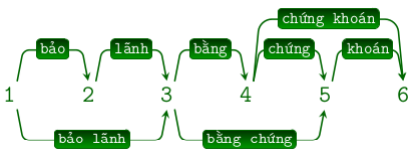
\includegraphics[scale=0.5]{vietnam_sentence.png}
\centering
\caption{\textit{The ambiguous in Vietnamese word segmentation}}
\end{figure}

In this example, there are more than one way to understanding
this sentence corresponding to two word segmentation
results:
\begin{enumerate}
  \item \enquote{Bảo\_lãnh bằng chứng\_khoán} and this mean is \enquote{\textbf{\textit{Guarantee by stock}}}.
  \item \enquote{Bảo\_lãnh bằng\_chứng khoán} is a meaningless sentence.
\end{enumerate}

The segmentation is an important step in text preprocessing
because if we segment words in the first way, we may classify
it in \enquote{\textit{finance market}}. However, if we segment words in the
second way, we may classify it to other category. Because our
approach in this paper is based on keywords extraction, the
accuracy of words segmentation progress is very important.
The failure in words segmentation synonymous with low
accuracy of keywords extraction after that.

After the keywords extraction phase, we have a dictionary
of keywords. We have used it to train new model for text
classification.

The rest of this paper is organized as follows: we discuss
the related works in the next section. Section 3 then presents some Machine Learning methods for 
Text Classification in Vietnamese news data. Section 4 gives the results of experiments we
conducted and Section 5 reports our conclusions and future works.

% needed in second column of first page if using \IEEEpubid
%\IEEEpubidadjcol

% An example of a floating figure using the graphicx package.
% Note that \label must occur AFTER (or within) \caption.
% For figures, \caption should occur after the \includegraphics.
% Note that IEEEtran v1.7 and later has special internal code that
% is designed to preserve the operation of \label within \caption
% even when the captionsoff option is in effect. However, because
% of issues like this, it may be the safest practice to put all your
% \label just after \caption rather than within \caption{}.
%
% Reminder: the "draftcls" or "draftclsnofoot", not "draft", class
% option should be used if it is desired that the figures are to be
% displayed while in draft mode.
%
%\begin{figure}[!t]
%\centering
%\includegraphics[width=2.5in]{myfigure}
% where an .eps filename suffix will be assumed under latex, 
% and a .pdf suffix will be assumed for pdflatex; or what has been declared
% via \DeclareGraphicsExtensions.
%\caption{Simulation Results}
%\label{fig_sim}
%\end{figure}

% Note that IEEE typically puts floats only at the top, even when this
% results in a large percentage of a column being occupied by floats.


% An example of a double column floating figure using two subfigures.
% (The subfig.sty package must be loaded for this to work.)
% The subfigure \label commands are set within each subfloat command, the
% \label for the overall figure must come after \caption.
% \hfil must be used as a separator to get equal spacing.
% The subfigure.sty package works much the same way, except \subfigure is
% used instead of \subfloat.
%
%\begin{figure*}[!t]
%\centerline{\subfloat[Case I]\includegraphics[width=2.5in]{subfigcase1}%
%\label{fig_first_case}}
%\hfil
%\subfloat[Case II]{\includegraphics[width=2.5in]{subfigcase2}%
%\label{fig_second_case}}}
%\caption{Simulation results}
%\label{fig_sim}
%\end{figure*}
%
% Note that often IEEE papers with subfigures do not employ subfigure
% captions (using the optional argument to \subfloat), but instead will
% reference/describe all of them (a), (b), etc., within the main caption.


% An example of a floating table. Note that, for IEEE style tables, the 
% \caption command should come BEFORE the table. Table text will default to
% \footnotesize as IEEE normally uses this smaller font for tables.
% The \label must come after \caption as always.
%
%\begin{table}[!t]
%% increase table row spacing, adjust to taste
%\renewcommand{\arraystretch}{1.3}
% if using array.sty, it might be a good idea to tweak the value of
% \extrarowheight as needed to properly center the text within the cells
%\caption{An Example of a Table}
%\label{table_example}
%\centering
%% Some packages, such as MDW tools, offer better commands for making tables
%% than the plain LaTeX2e tabular which is used here.
%\begin{tabular}{|c||c|}
%\hline
%One & Two\\
%\hline
%Three & Four\\
%\hline
%\end{tabular}
%\end{table}


% Note that IEEE does not put floats in the very first column - or typically
% anywhere on the first page for that matter. Also, in-text middle ("here")
% positioning is not used. Most IEEE journals use top floats exclusively.
% Note that, LaTeX2e, unlike IEEE journals, places footnotes above bottom
% floats. This can be corrected via the \fnbelowfloat command of the
% stfloats package.


\section{Related works}
\subsection{Text Classification}
\textit{\textbf{Text classification}} is the process of assigning text documents to one or more predefined
categories or classes. This is not a new problem. Actually, as early as the 1800s, Knowledge Engineering (KF) techniques are used to create the automatic document
classifiers in their manual construction. Nowadays, when Machine Learning (\textbf{\textit{ML}}) becomes a trending vision, \textbf{\textit{ML}} methods are used in a wide variety of domains for the purposes of classification. Of course, it's can apply to solve \textbf{\textit{TC}}. In \textbf{\textit{ML}} we can consider this problem with a multiclass classification problem. In basically, automatic text classification uses a corpus and we extract some kind of features for each of the texts. Then we apply a mathematical model, a classifier, which somehow estimates the similarities between different texts based on the features, and guesses this category. We have some methods to approach and many of them can be directly applied to news classification as long as there exists a good
training corpus [5, 6]. The most of them are \textit{Naive Bayes} (\textbf{\textit{NB}}) [9], \textit{Support Vector Machine} (\textbf{\textit{SVM}}) [8] and Convolutional Neural Network (\textbf{\textit{CNN}}) [10] is a state-of-the-art for English processing. The \textit{\textbf{TC}} process is simulate in \textbf{\textit{Fig 2}} below:

\begin{figure}[h]
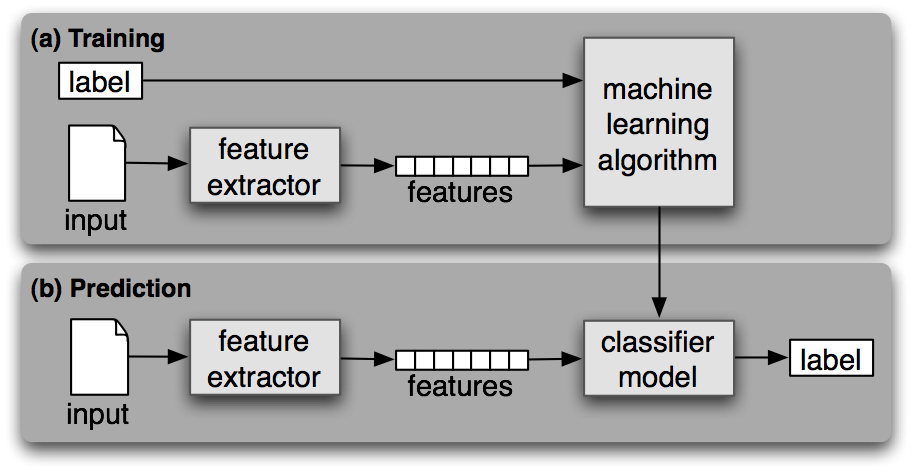
\includegraphics[scale=0.57]{workflow.png}
\centering
\caption{\textit{Text Classification Process}}
\end{figure}

\subsection{Vietnamese Corpus}
Some research in English \textbf{\textit{TC}} has generally achieved satisfactory results with the
results on some standard corpora such as Reuters and 20 Newsgroups ranging from 80 to 93\% of accuracy [12]. However, the Vietnamese datasets are very restricted and small (from 50 to 100 files per topic) which are not available publicly for independent research [13]. Really fortunately in the research of Vu Cong Duy and colleagues [11] had constructed a Vietnamese corpus which satisfies the conditions of sufficiency, objectiveness and balance. We had used this corpus for research in current paper. Below is the detailed description of the corpus.

This corpus based on the four largest circulation Vietnamese online newspapers: VnExpress\footnote{\url{www.vnexpress.net}}, TuoiTre Online\footnote{\url{www.tuoitre.com.vn}}, Thanh Nien Online\footnote{\url{www.thanhnien.com.vn}}, Nguoi Lao Dong Online\footnote{\url{www.nld.com.vn}}
The collected texts are automatically preprocessed
(removing the HTML tags, spelling normalization) by Teleport
software and manual correction by linguists who reviewed and adjusted the documents which are
classified to the wrong topics. Finally, they obtained a relatively large and sufficient corpus includes top categories. Level 1 of this corpus contains about 33,759 documents for training and 50,373 documents for testing. Two part of the dataset is shown on \textit{\textbf{Fig 3}} and \textit{\textbf{Fig 4}}.

\begin{figure}[h]
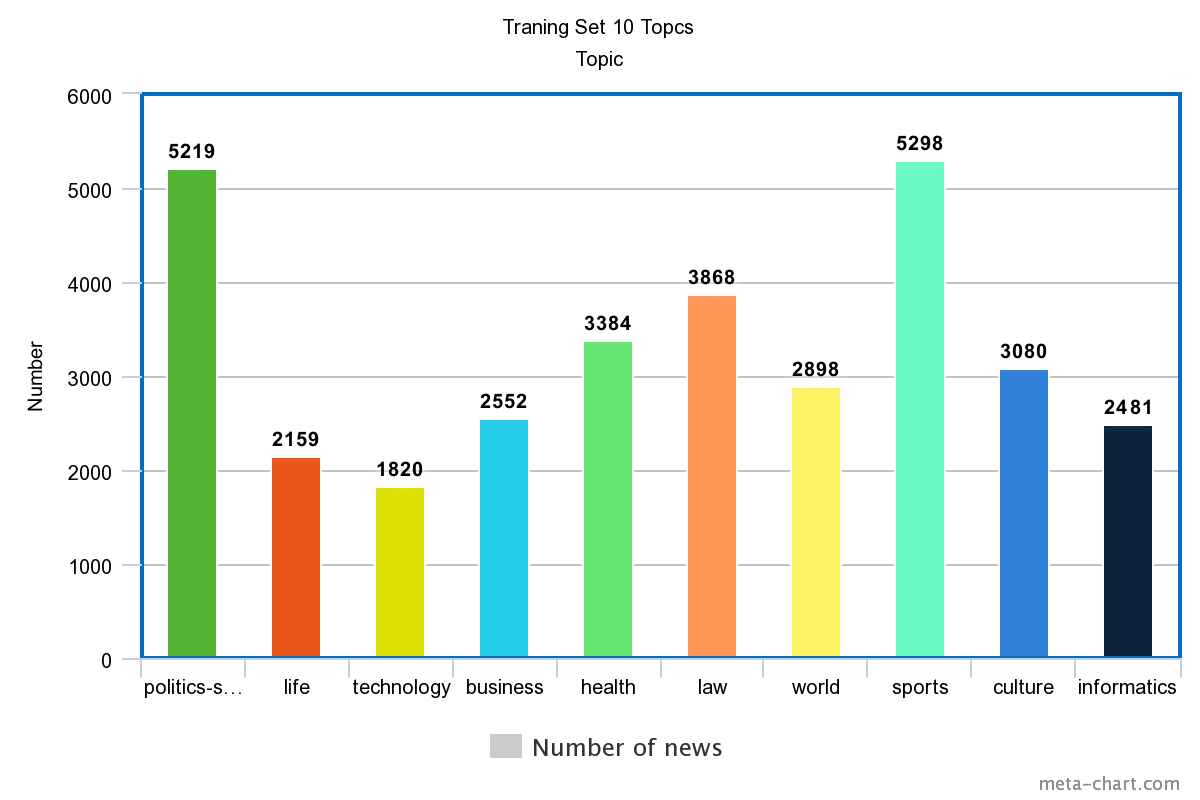
\includegraphics[scale=0.2]{training_10.png}
\centering
\caption{\textit{Training set in 10 topic corpus}}
\end{figure}

\begin{figure}[h]
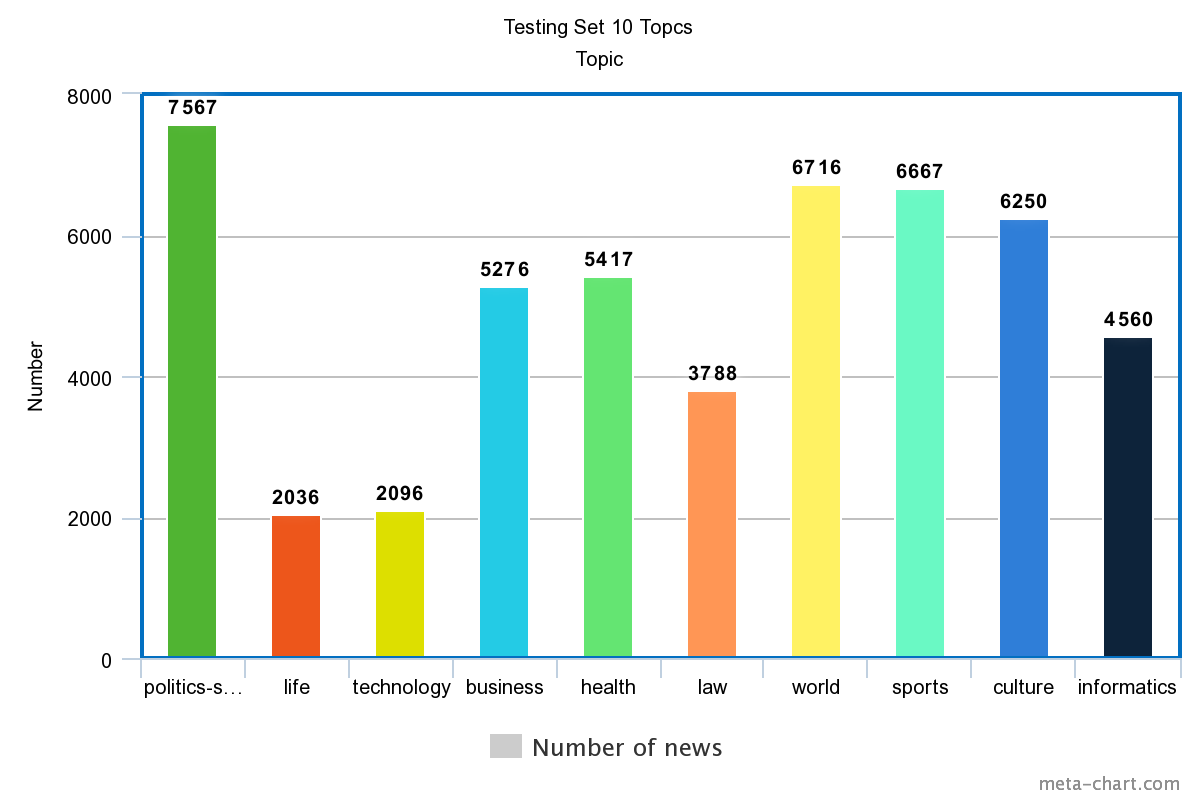
\includegraphics[scale=0.2]{testing_10.png}
\centering
\caption{\textit{Testing set in 10 topic corpus}}
\end{figure}

Another variant of this dataset have 27 topics. The topics which are child topics of the corpus above. 
The division in the Level 1 is very vague meanwhile and they need to find a specific topic to experiment for TC [11]. We used both two level of dataset in this paper to training the Vietnamese text classifier.
\subsection{Keyword Extraction}
\textit{Keyword extraction} is an important technique for document
retrieval, text classification, document clustering, text summarization, etc. By extracting appropriate keywords, we can choose easily which document to read or learn the relation among documents and we can apply this method for reduce the demension of input space in our \textit{\textbf{TC}} problem. Extract a keywords set in a text document is finding unique words. The unique words are the words that
has no duplication and not included in stop words list and keywords and their frequency are ordered
by descending weight. We take ten top keywords to be calculated \textit{Keyword Score} by using equation below:

\begin{equation}
KeywordScore(k_i)=1.5 \frac{\abs{k_i}}{\abs{W}}
\end{equation}

Where $k_i$ that will be calculated and $\abs{k_i}$ is the frequency of keywords occurrence in the text, and $\abs{W}$ is the number of unique keywords in the text. We extract top keywords of a article after each keyword has its score and \textit{build a dictionary} of keywords in all documents of our corpus. 

\subsection{Feature Selection}
\subsubsection{Bag of Words Approach}
Before any classification task, a important task is that of document representation and feature
selection. Actually, we have two ways can be used to represent a text document are \textit{Bag of Words - BoW} and represent text directly as strings. Most text classification
methods use the \textit{\textbf{BoW}} representation because of its simplicity
for classification purposes. In \textit{\textbf{BoW}} method, a document is represented as a set of
words, together with their associated frequency in the document. Such a representation is essentially independent of the sequence of words in the collection. Words can be made from one morpho-syllable, or
many morpho-syllables.
\subsubsection{Word Segmentation}
So in this approach, a robust solution to document classification requires a good Vietnamese word segmentation module. We use \textit{\textbf{vnTokenizer}} [15] - the state-of-the-art word segmentation program in the \textbf{\textit{BoW}} approach. Text documents are segmented into words or tokens before create a dictionary in preprocessing. 
\subsubsection{Stop-words Removal}
The most common feature selection is that of \textit{\textbf{stop-words}} removal and stemming.
In stop-words removal, we determine the common words in the documents
which are not specific or discriminatory to the different classes. Defined
words (e.g., \enquote{và}, \enquote{bị} and \enquote{chính là}) are ignored in text processing. For this purpose, we  prepared a stop-words list (about $\approx$2000 words, collected manually). 

% if have a single appendix:
%\appendix[Proof of the Zonklar Equations]
% or
%\appendix  % for no appendix heading
% do not use \section anymore after \appendix, only \section*
% is possibly needed

% use appendices with more than one appendix
% then use \section to start each appendix
% you must declare a \section before using any
% \subsection or using \label (\appendices by itself
% starts a section numbered zero.)
%
\section{Text classification methods}
After text preprocessing above, we have numeric training features from the Bag of Words and the original categories for each feature vector. We can apply some supervised learning algorithms to solve the text classification. In this paper, we consider some multiclass classification algorithms and compared with our Neural Network Architecture. Some methods as \textbf{\textit{Random Forest}}, \textit{\textbf{Support Vector Machine}} will be represented below.

\subsection{Random Forest}
\textit{\textbf{Random Forest - RF}} is a famous algorithm for classification in Machine Learning. A \textit{Random Forest} is a classifier consisting of a collection of tree-structured classifier $\{RF(x, \theta_k), k=1,...\}$ where $(\theta_k)$ are independent identically distributed random vectors and each tree casts a unit vote for the most popular class at input $x$ [16]. This classifier use averaging to improve the predictive accuracy and control over-fitting. Actually, \textbf{RF} is a meta estimator that fits a number of decision tree classifiers on various sub-samples of the dataset. 

For classification problems, given a set of simple trees and a set of random predictor variables, the \textbf{RF} method defines a margin function that measures the extent to which the average number of votes for the correct class exceeds the average vote for any other class present in the dependent variable. Given a set of classifier denoted with \[RF_1(x), RF_2(x),..., RF_k(x)\]
the features vector \textbf{X} and the labels vector \textbf{y}. The margin function \textit{M} is defined as: 
\[M(X,y)=avI(h_k(X)=y)-max_{j\neq y}avI(h_k(X)=j)\]
where $I$ is the indicator function. This measure provides us not only with a convenient way of making predictions, but also with a way of associating a confidence measure with those predictions. 

The predictions of the Random Forest are taken to be the average of the predictions of the trees:
\[s=\frac{1}{N}\sum_{i=1}^{N}s_i\]
where $s_i$ is the prediction of tree $i$. The index $i$ runs over the individual trees in the forest.

\textit{RF} can flexibly incorporate missing data in the predictor variables. When missing data are encountered for a particular observation during model building, the prediction made for that case is based on the last preceding node in the respective tree. 
\subsection{Support Vector Machines}
\textbf{\textit{Support Vector Machines - SVMs}} were first proposed in [17 18] for numerical data. The main principle of SVMs is to determine separators in the search space which can best separate the different classes. For example,
consider the example illustrated in \textit{\textbf{Fig 5}} below
\begin{figure}[h]
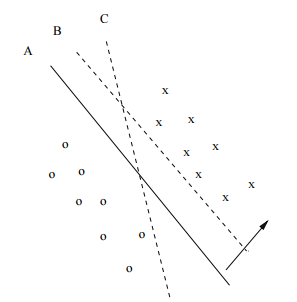
\includegraphics[scale=0.45]{svm.png}
\centering
\caption{\textit{Best separating hyperplane selection in SVM}}
\end{figure}

In which we have two classes denoted by \enquote*{\textbf{x}} and \enquote*{\textbf{o}} respectively. We have denoted three different separating hyperplanes, which are denoted by \textbf{A}, B\textbf{,} and \textbf{C} respectively.
It is evident that the hyperplane \textbf{A} provides the best separation
between the different classes, because the normal distance of any of the
data points from it is the largest. Therefore, the hyperplane \textbf{A} represents
the maximum margin of separation. We note that the normal vector to
this hyperplane (represented by the arrow in the figure) is a direction in
the feature space along which we have the maximum discrimination. 

In this problem,  numbers of classes is more than two - \textit{multiclass problem}. Assume that we have a set of \textit{m} training example $S=\left \{ (x_1, y_1),..,(x_m, y_m) \right \}$
with $x_i$ is the feature vector $i^{th}$ and $y_i$ is respective label. We assume that each example $x_i$ is drawn from a domain $X\subseteq R^n$ and that each label $y_i$ i is an integer from the set $Y=\left \{ 1..k \right \}$ with $k$ is the numbers of classes. A \textbf{\textit{multiclass}} classifier is a fucntion $H:X\rightarrow Y$ that maps an instance $x$ - in this problem is the \textit{BoW feature vector} to an label $y$ in $Y$ [19]: 

\[H_M(x)=arg \max_{1}^{k}(M_r.x)\]
where $M$ is the matrix of size $k\times n$ over $R$ and $M_r$ is $r^{th}$ of $M$. We interchangeably
call the value of the inner-product of the $r^{th}$ row of $M$ with the instance $x$ the \textit{confidence}
and the \textit{similarity score} for the $r$ class. With the definition above,  the
predicted label is the index of the row attaining the highest similarity score with $x$.Our problem have $k\geq 3$ in which we maintain $k$ prototypes $M_1, M_2,..., M_k $ and set the label of a new input instance by choosing the index
of the most similar row of $M$.

\subsection{Neural Network}
The basic idea of neural network is a \textit{neuron} in which each neurol receives a set of inputs denoted by vector $\overline{X}_i$. In this case, $\overline{X}_i$ correspond to the \textit{BoW feature vector} in the $i^{th}$ document. Each neuron is also associated with a set of weights \textit{W}, which are used in order to compute a function \textit{f(·)} of its inputs. The sign of the predicted function $p_i$ yields the class label of vector $\overline{X}_i$ A typical function which is often used in the neural network is the \textit{linear function} as follows:
\[p_i=W.\overline{X}_i\]

For the multi-class problem, the neural-network can be described formally as follows.	 With \textit{d} is the lenght of dictionary after \textit{BoW} preprocessing. For a given \textit{d}-dimensional feature space $X$, the training dataset denoted by $X_{tr}$ and  each element $\overline{x}\in X_{tr}$ is associated with a class label $y_i$ of the label $Y$. A neural network system $F$ can be trained on $S_{tr}$ such that for any given feature vector $\overline{x}\in X$ and 	$F(\overline{x})\in Y$. \textit{F} can be a system of neural networks or a single neural network whose weights. In this paper, we use a multi-layered feed forward neural network. We
denote the input and output at a hidden node \textit{j} as:
\[f_{j}^{h}=\sum_{i}w_{ji}^{h}x_i\]
with $j=1...H$ where $x_i$ is the $i^{th}$ input of feature vector 	$\overline{x}$, and $w_{ji}^{h}$ is the weight
associated with the input $x_i$ to the $j^{th}$ hidden node. $H$ is the number of hidden node. We applied a activation fucntion denoted by $g^h(.)$  in the hidden layer. Some of activation fucntion as \textit{Sigmoid} [21], \textit{ReLU} [22], \textit{Softmax} [22]... The output value from the $j^{th}$ hidden unit denoted by $z_j=g^h(f_{i}{h})$. In the output layer, each node $O_k$ has the input and output as follows:
\[f_{k}^{o}=\sum_{i}w_{kj}^{o}z_j\]. Finally we have the label class associate with feature vector $\overline{x}_k$
\[y_k=g^o(j_{k}^{o})\]
$k=1...M$ with \textit{M} is the number of the output nodes.

In this paper, we create a network with 6 hidden layers with the \textit{\textbf{tanh}} activation function [24] and used \textit{stochastic gradient descent} [23] to optimization in this network. The input layer is the feature vector after feature seletion pharse with \textit{\textbf{BoW}} method and the output layer is label vector of the documents. The simulation of network architecture is present in \textbf{\textit{Fig 6}}

\begin{figure}[h]
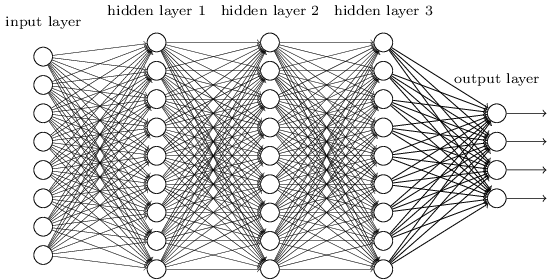
\includegraphics[scale=0.45]{dense.png}
\centering
\caption{\textit{Simulation of Neural Network architecture}}
\end{figure}
\section{Result}
Two recall and precision parameters are used to evaluate the classification models [25]. The $Recall$ is defined as below:
\[Recall=\frac{\sum_{d\in D}d_{TrueModel}}{\sum_{d\in D}d_{Practice}}\]
and $Precision$ as
\[Precision=\frac{\sum_{d\in D}d_{TrueModel}}{\sum_{d\in D}d_{AllModel}}\]
In that:
\begin{itemize}
  \item The $d_{TrueModel}$ is the number of documents classified by the model correctly.
  \item The $d_{AllModel}$ is the number of documents classified by the model.
  \item The $d_{Practice}$ is the number of documents classified correctly in practice.
\end{itemize}
The $F_1$ score is calculated with:
\[F_1=\frac{2.Recall.Precision}{Recall + Precision}\]

Our \textit{Keyword extraction with BoW} method is abbreviated with \textit{\textbf{KEBoW}}. We investigate the comparison with \textit{\textbf{N-gram}} method introducted in the research of Vu Cong Duy [11], and difference Machine Learning algorithms as \textit{\textbf{SVMs multiclass, Random Forest, SVC}}. Additionally, the total accuracy is calculated from the average accuracy of all categories for each experiment. The result is present with some figures \textit{\textbf{Fig 7, Fig 8}} and \textit{\textbf{Fig 9}}

\begin{figure}[h]
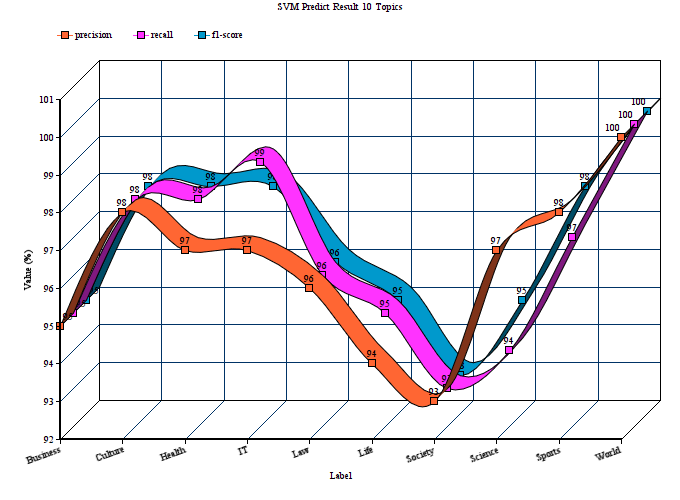
\includegraphics[scale=0.45]{svm_predict.png}
\centering
\caption{\textit{Prediction Result with SVM 10 Topics dataset}}
\end{figure}

\begin{figure}[h]
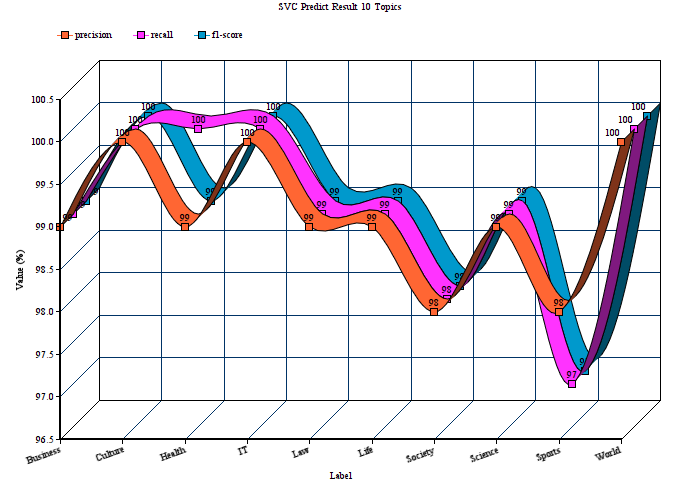
\includegraphics[scale=0.45]{svc_predict.png}
\centering
\caption{\textit{Prediction Result with SVC 10 Topics dataset}}
\end{figure}

\begin{figure}[h]
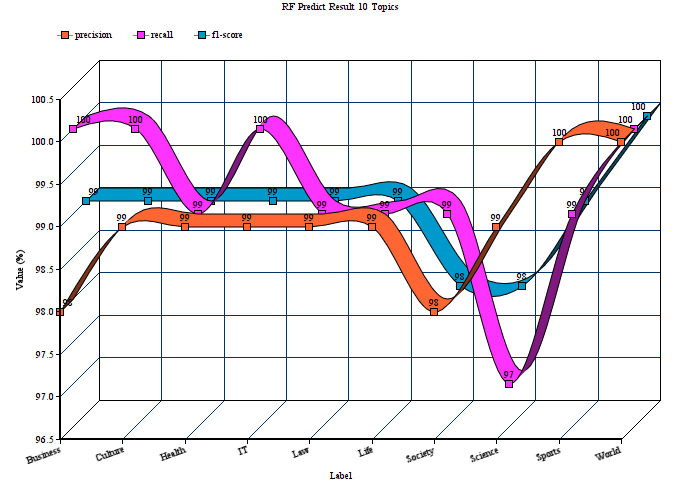
\includegraphics[scale=0.45]{random_forest_predict.png}
\centering
\caption{\textit{Prediction Result with Random Forest 10 Topics dataset}}
\end{figure}

\begin{figure}[h]
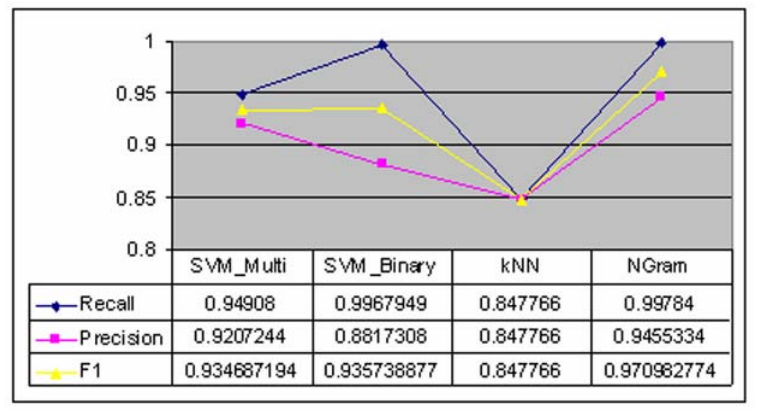
\includegraphics[scale=0.3]{level_1_other.png}
\centering
\caption{\textit{Best prediction result in other paper [11]}}
\end{figure}
The \textit{\textbf{Fig 7, Fig 8}} and \textit{\textbf{Fig 9}} showed that the prediction result of respective algorithms with \textbf{\textit{KEBoW}} extraction method with \textit{\textbf{10 Topics dataset}}. We can see the best result of other research [11] with current dataset in \textit{\textbf{Fig 10}}. Easy to see that our prediction result better than the result in \textit{\textbf{Fig 10}} in the same dataset. It proves that our feature selection method with keywords extraction and BoW have more effective other features selection methods.

However, we are only improved the features selection pharse with \textit{\textbf{KEBoW}} method, but also we proposed a Neural Network applied in the training pharse. The comparison of our Neural Network accuracy with some algorithms is shown in \textit{\textbf{Table 1}}.
\begin{table}[]
\centering
\caption{\textit{Accuracy Comparsion Result}}
\label{my-label}
\begin{tabular}{|l|l|l|l|l|}
\hline
                                                           & {\color[HTML]{333333} \textit{\textbf{SVM}}} & {\color[HTML]{333333} \textit{\textbf{Random Forest}}} & {\color[HTML]{333333} \textit{\textbf{SVC}}} & {\color[HTML]{333333} \textit{\textbf{Neural Network}}} \\ \hline
{\color[HTML]{333333} \textit{\textbf{10 Topics Dataset}}} & 0.9652                                       & 0.9921                                                 & 0.9922                                       & 0.9975                                                  \\ \hline
{\color[HTML]{333333} \textit{\textbf{27 Topics Dataset}}} & 0.9780                                       & 0.9925                                                 & 0.9965                                       & 0.9969                                                  \\ \hline
\end{tabular}
\end{table}

\section{Conclusion and future works}
With the difference between Vietnamese and other languages, the research to find a feasible approach for Vietnamese text classification is the new challenge of us. By our experiments, we proposed new neural network architecture with average accuracy 99.75\%. This result is much better than some methods as \textit{\textbf{SVM}}, \textbf{\textit{Random Forest}} in the same dataset. Especially our result achieved is better than the research of Vu Cong Duy [11] with the same algorithm in the same dataset. It proves that our feature selection method with keywords extraction and BoW have more effective other features selection methods.

However, we also recognize that these approaches for Vietnamese TC occur some errors such as:  
\begin{enumerate}
  \item The stopwords list is builded from subjective views and it maybe not have high accuracy
  
  \item The corpus have the ambiguities between two or many topics.
  \item The segmentation is limited by third-party library.
\end{enumerate}

In the future, we could improve the accuracy of our Neural Network, overcome the disvantages of preprocessing pharse and combine more semantic and contextual features in this text classification problem for Vietnamse. 
\section*{Application of Research}
The research result was applied in Viblo post automatic \footnote{\url{www.viblo.asia}} - a free service for technical knowledge sharing of \textbf{\textit{Framgia Vietnam}}\footnote{\url{www.recruit.framgia.vn}}

\section*{Acknowledgment}


This research was partially supported by \textbf{\textit{Framgia Vietnam}}. We are thankful to our colleagues who provided  expertise that greatly assisted the research, although they may not agree with all of the interpretations provided in this paper.


% Can use something like this to put references on a page
% by themselves when using endfloat and the captionsoff option.
\ifCLASSOPTIONcaptionsoff
  \newpage
\fi



% trigger a \newpage just before the given reference
% number - used to balance the columns on the last page
% adjust value as needed - may need to be readjusted if
% the document is modified later
%\IEEEtriggeratref{8}
% The "triggered" command can be changed if desired:
%\IEEEtriggercmd{\enlargethispage{-5in}}

% references section

% can use a bibliography generated by BibTeX as a .bbl file
% BibTeX documentation can be easily obtained at:
% http://www.ctan.org/tex-archive/biblio/bibtex/contrib/doc/
% The IEEEtran BibTeX style support page is at:
% http://www.michaelshell.org/tex/ieeetran/bibtex/
%\bibliographystyle{IEEEtran}
% argument is your BibTeX string definitions and bibliography database(s)
%\bibliography{IEEEabrv,../bib/paper}
%
% <OR> manually copy in the resultant .bbl file
% set second argument of \begin to the number of references
% (used to reserve space for the reference number labels box)
\begin{thebibliography}{1}

\bibitem{1}
BLOM, ALEXANDER, and SOFIE THORSEN. "A sentiment-based chat bot." (2013).
\bibitem{2}
Mooney, Raymond J., and Loriene Roy. "Content-based book recommending using learning for text categorization." Proceedings of the fifth ACM conference on Digital libraries. ACM, 2000.
\bibitem{3}
Dien, Dinh, and Vu Thuy. "A maximum entropy approach for Vietnamese
word segmentation." Research, Innovation and Vision for the Future,
2006 International Conference on. IEEE, 2006.
\bibitem{4}
 D.Dien, H.Kiem, and N.V.Toan, “Vietnamese Word Segmentation”.
2001. Proceedings of NLPRS’01. The 6th Natural Language Processing
Pacific Rim Symposium, Tokyo, Japan, 11/2001, pp.749-756, 2001
\bibitem{5}
Y. Yang and X. Liu. A re-examination of text categorization methods. In 22nd
Annual International SIGIR, pages 42–49, Berkley, August 1999.
\bibitem{6}
F. Sebastiani. Machine learning in automated text categorisation: a survey. Technical
Report IEI-B4-31-1999, Istituto di Elaborazione dell’Informazione, Consiglio
Nazionale delle Ricerche, Pisa, IT, 1999. Revised version, 2001
\bibitem{7}
Yang, Y. 1994. Expert network: effective and efficient learning from
human decisions in text categorization and retrieval. In Proceedings of
SIGIR-94, 17th ACM International Conference on Research and
Development in Information Retrieval (Dublin, IE, 1994), pp. 13–22.
\bibitem{8}
Thorsten Joachims. Text Categorization with Support Vector Machines:
Learning with Many Relevant Features. In C. Nedellec and C.
Rouveirol, editors, Proceedings of ECML-98, 10th European
Conference on Machine Learning, number 1398, pages 137—142.
\bibitem{9}
Shimodaira, Hiroshi. "Text classificckation using naive bayes." Learning and Data Note 7 (2014): 1-9.
\bibitem{10}
Zhang, Xiang, Junbo Zhao, and Yann LeCun. "Character-level convolutional networks for text classification." Advances in neural information processing systems. 2015.
\bibitem{11}
Hoang, Vu Cong Duy, et al. "A comparative study on vietnamese text classification methods." Research, Innovation and Vision for the Future, 2007 IEEE International Conference on. IEEE, 2007.
\bibitem{12}
Sebastiani, Fabrizio. "Machine learning in automated text categorization." ACM computing surveys (CSUR) 34.1 (2002): 1-47.
\bibitem{13}
Hung Nguyen, Ha Nguyen, Thuc Vu, Nghia Tran, and Kiem Hoang.
2005. Internet and Genetics Algorithm-based Text Categorization for
Documents in Vietnamese. Proceedings of 4th IEEE International
Conference on Computer Science - Research, Innovation and Vision of
the Future 2006 (RIVF’06). Ho Chi Minh City, Vietnam , Feb 12-16,
2006
\bibitem{14}
Gunawan, D., et al. "Automatic Text Summarization for Indonesian Language Using TextTeaser." IOP Conference Series: Materials Science and Engineering. Vol. 190. No. 1. IOP Publishing, 2017.
\bibitem{15}
Le, Ngoc Minh, et al. "VNLP: an open source framework for Vietnamese natural language processing." Proceedings of the Fourth Symposium on Information and Communication Technology. ACM, 2013.
\bibitem{16}
Breiman, Leo. "Random forests." UC Berkeley TR567 (1999).
\bibitem{17}
V. Vapnik. Estimations of dependencies based on statistical data,
Springer, 1982.
\bibitem{18}
C. Cortes, V. Vapnik. Support-vector networks. Machine Learning,
20: pp. 273–297, 1995.
\bibitem{19}
Crammer, Koby, and Yoram Singer. "On the algorithmic implementation of multiclass kernel-based vector machines." Journal of machine learning research 2.Dec (2001): 265-292.
\bibitem{20}
Ou, Guobin, and Yi Lu Murphey. "Multi-class pattern classification using neural networks." Pattern Recognition 40.1 (2007): 4-18.
\bibitem{21}
Yin, Xinyou, et al. "A flexible sigmoid function of determinate growth." Annals of botany 91.3 (2003): 361-371.
\bibitem{22}
Glorot, Xavier, Antoine Bordes, and Yoshua Bengio. "Deep sparse rectifier neural networks." Proceedings of the Fourteenth International Conference on Artificial Intelligence and Statistics. 2011.
\bibitem{23}
Bottou, Léon. "Large-scale machine learning with stochastic gradient descent." Proceedings of COMPSTAT'2010. Physica-Verlag HD, 2010. 177-186.
\bibitem{24}
Karlik, Bekir, and A. Vehbi Olgac. "Performance analysis of various activation functions in generalized MLP architectures of neural networks." International Journal of Artificial Intelligence and Expert Systems 1.4 (2011): 111-122.
\bibitem{25}
Fabrizio Sebastiani. 2002. Machine Learning in Automated Text
Categorization. ACM Computing Surveys, Vol. 34, No. 1, March 2002,
pp.1- 47 
\bibitem{26}
Salih, A. M., et al. "Modified extraction 2-thiobarbituric acid method for measuring lipid oxidation in poultry." Poultry Science 66.9 (1987): 1483-1488.
\end{thebibliography}


% biography section
% 
% If you have an EPS/PDF photo (graphicx package needed) extra braces are
% needed around the contents of the optional argument to biography to prevent
% the LaTeX parser from getting confused when it sees the complicated
% \includegraphics command within an optional argument. (You could create
% your own custom macro containing the \includegraphics command to make things
% simpler here.)
%\begin{biography}[{\includegraphics[width=1in,height=1.25in,clip,keepaspectratio]{mshell}}]{Michael Shell}
% or if you just want to reserve a space for a photo:

\begin{IEEEbiography}[{\includegraphics[width=1in,height=1.25in,clip,keepaspectratio]{picture}}]{John Doe}
\blindtext
\end{IEEEbiography}

% You can push biographies down or up by placing
% a \vfill before or after them. The appropriate
% use of \vfill depends on what kind of text is
% on the last page and whether or not the columns
% are being equalized.

%\vfill

% Can be used to pull up biographies so that the bottom of the last one
% is flush with the other column.
%\enlargethispage{-5in}



% that's all folks
\end{document}


